\documentclass{report}
\usepackage{a4}
\usepackage[latin1]{inputenc}
%\usepackage[dvips]{graphicx}
\usepackage[pdftex]{graphicx}
\usepackage{verbatim}
\usepackage[total={6in, 9in}, top=1in,left=1.1in]{geometry} 
\usepackage{moreverb}
\usepackage{psfrag}
\usepackage{amsmath}
\usepackage[small]{caption}
\usepackage{amssymb}
\usepackage{fancyhdr}
\usepackage{shadow}            
\usepackage{setspace}
\usepackage{listings}
\usepackage{subfig}
\usepackage{upquote} %To make straigh quotes work in pdf

\setlength{\headheight}{12.5pt}
\newcommand{\undertilde}[1]{\underset{\widetilde{}}{#1}}
\newcommand{\HRule}{\rule{\linewidth}{0.5mm}}

\pagestyle{fancy}


\begin{document}

\begin{titlepage}
  \begin{center}
 

    {\small Cite as: Carlsson, P.: A dieselFoam tutorial. In Proceedings of CFD with OpenSource Software, 2008, Edited by Nilsson. H., \verb+http://www.tfd.chalmers.se/~hani/kurser/OS_CFD_2008+}
	
	~\\[0.4cm]
	\textsc{\LARGE CFD with OpenSource software}\\[0.5cm]	
	\textsc{A course at Chalmers University of Technology}\\
	\textsc{Taught by H{\aa}kan Nilsson}\\[0.5cm]	
	
	\HRule \\[0.4cm]
	{ \huge \bfseries A dieselFoam tutorial}\\[0.4cm]
	\HRule \\[1cm]
	
        \begin{minipage}{0.35\textwidth}
        Developed for OpenFOAM-1.5.x\\
        Requires: PyFoam
	\end{minipage}\\[1cm]

	\begin{minipage}{0.4\textwidth}
	\begin{flushleft} \large
	\emph{Author:}\\
	Per \textsc{Carlsson}\\
        University of NN\\
        my.name@provider.com\\
        (if you like - or remove)
	\end{flushleft}
	\end{minipage}
	\begin{minipage}{0.4\textwidth}
	\begin{flushright} \large
	\emph{Peer reviewed by:} \\
	 \textsc{NaiXian Lu}\\
	\textsc{H\aa kan Nilsson}\\
	\end{flushright}
	\end{minipage}

        ~\\[1cm]

        Licensed under CC-BY-NC-SA, https://creativecommons.org/licenses/

	\vfill

        {Disclaimer: This is a student project work, done as part of a course where OpenFOAM and some other OpenSource software are introduced to the students. Any reader should be aware that it might not be free of errors. Still, it might be useful for someone who would like learn some details similar to the ones presented in the report and in the accompanying files. The material has gone through a review process. The role of the reviewer is to go through the tutorial and make sure that it works, that it is possible to follow, and to some extent correct the writing. The reviewer has no responsibility for the contents.}\\[2cm]

	{\large \today}
	 
	\end{center}

 \end{titlepage}

\chapter*{Learning outcomes}

The main requirements of a tutorial is that it should teach the four points: How to use it, The theory of it, How it is implemented, and How to modify it. Therefore the list of learning outcomes is organized with those headers.\\[0.4cm]

\noindent The reader will learn:\\[0.4cm]

\noindent{\bf How to use it:}
\begin{itemize}
\item how to use the dieselFoam solver.
\item ...
\end{itemize}
{\bf The theory of it:}
\begin{itemize}
\item the theory of ...
\item ...
\end{itemize}
{\bf How it is implemented:}
\begin{itemize}
\item ...
\end{itemize}
{\bf How to modify it:}    
\begin{itemize}
\item ...
\end{itemize}

\chapter*{Prerequisites}

The reader is expected to know the following in order to get maximum benefit out of this report:
\begin{itemize}
\item Fundementals of Heat and mass Tranfer , Book by Frank.P Incropera
\item Dimensional groups like Sherwood number,Reynolds,Number,Prandtl Number, Schmidt Num-
ber and Lewis Number
\item Run standard document tutorials like damBreak tutorial
\item It is strongly recommonded to gain a brief insight into the physics of two phase reactive flows
from the following journal (if accessable):\\
D. Darmana et.al.,2007. Detailed modelling of hydrodynamics, mass transfer and chemical
reactions in a bubble column using a discrete bubble model: Chemisorption of CO 2 into NaOH
solution, numerical and experimental study.Chemical Engineering Science 62,2556 to 2575
\end{itemize}

\tableofcontents

\chapter{Tutorial dieselFoam}

\section{Introduction}

This tutorial describes how to pre-process, run and post-process a case involving compressible reacting flow with Lagrangian evaporating particles in a three-dimensional domain. It also describes how to copy the solver, copy an evaporation model and how to add a second material to the discrete particles. 
\newline \newline
The geometry consists of a block filled with air, with a 0.01x0.01 meter base and a length of 0.1 meter (figure \ref{geo1}). An injector is centrally placed on the top boundary where n-Heptane ($C_7H_{16}$) is injected. When the discrete droplets enter the domain they evaporate and combustion takes place in the gas phase. There are several gas phase reaction schemes supplied with the case  ranging from a reaction scheme with 5 species and one reaction up to a reaction scheme involving $\sim$300 reactions and 56 species.    
\begin{figure}[h]
  \centering
  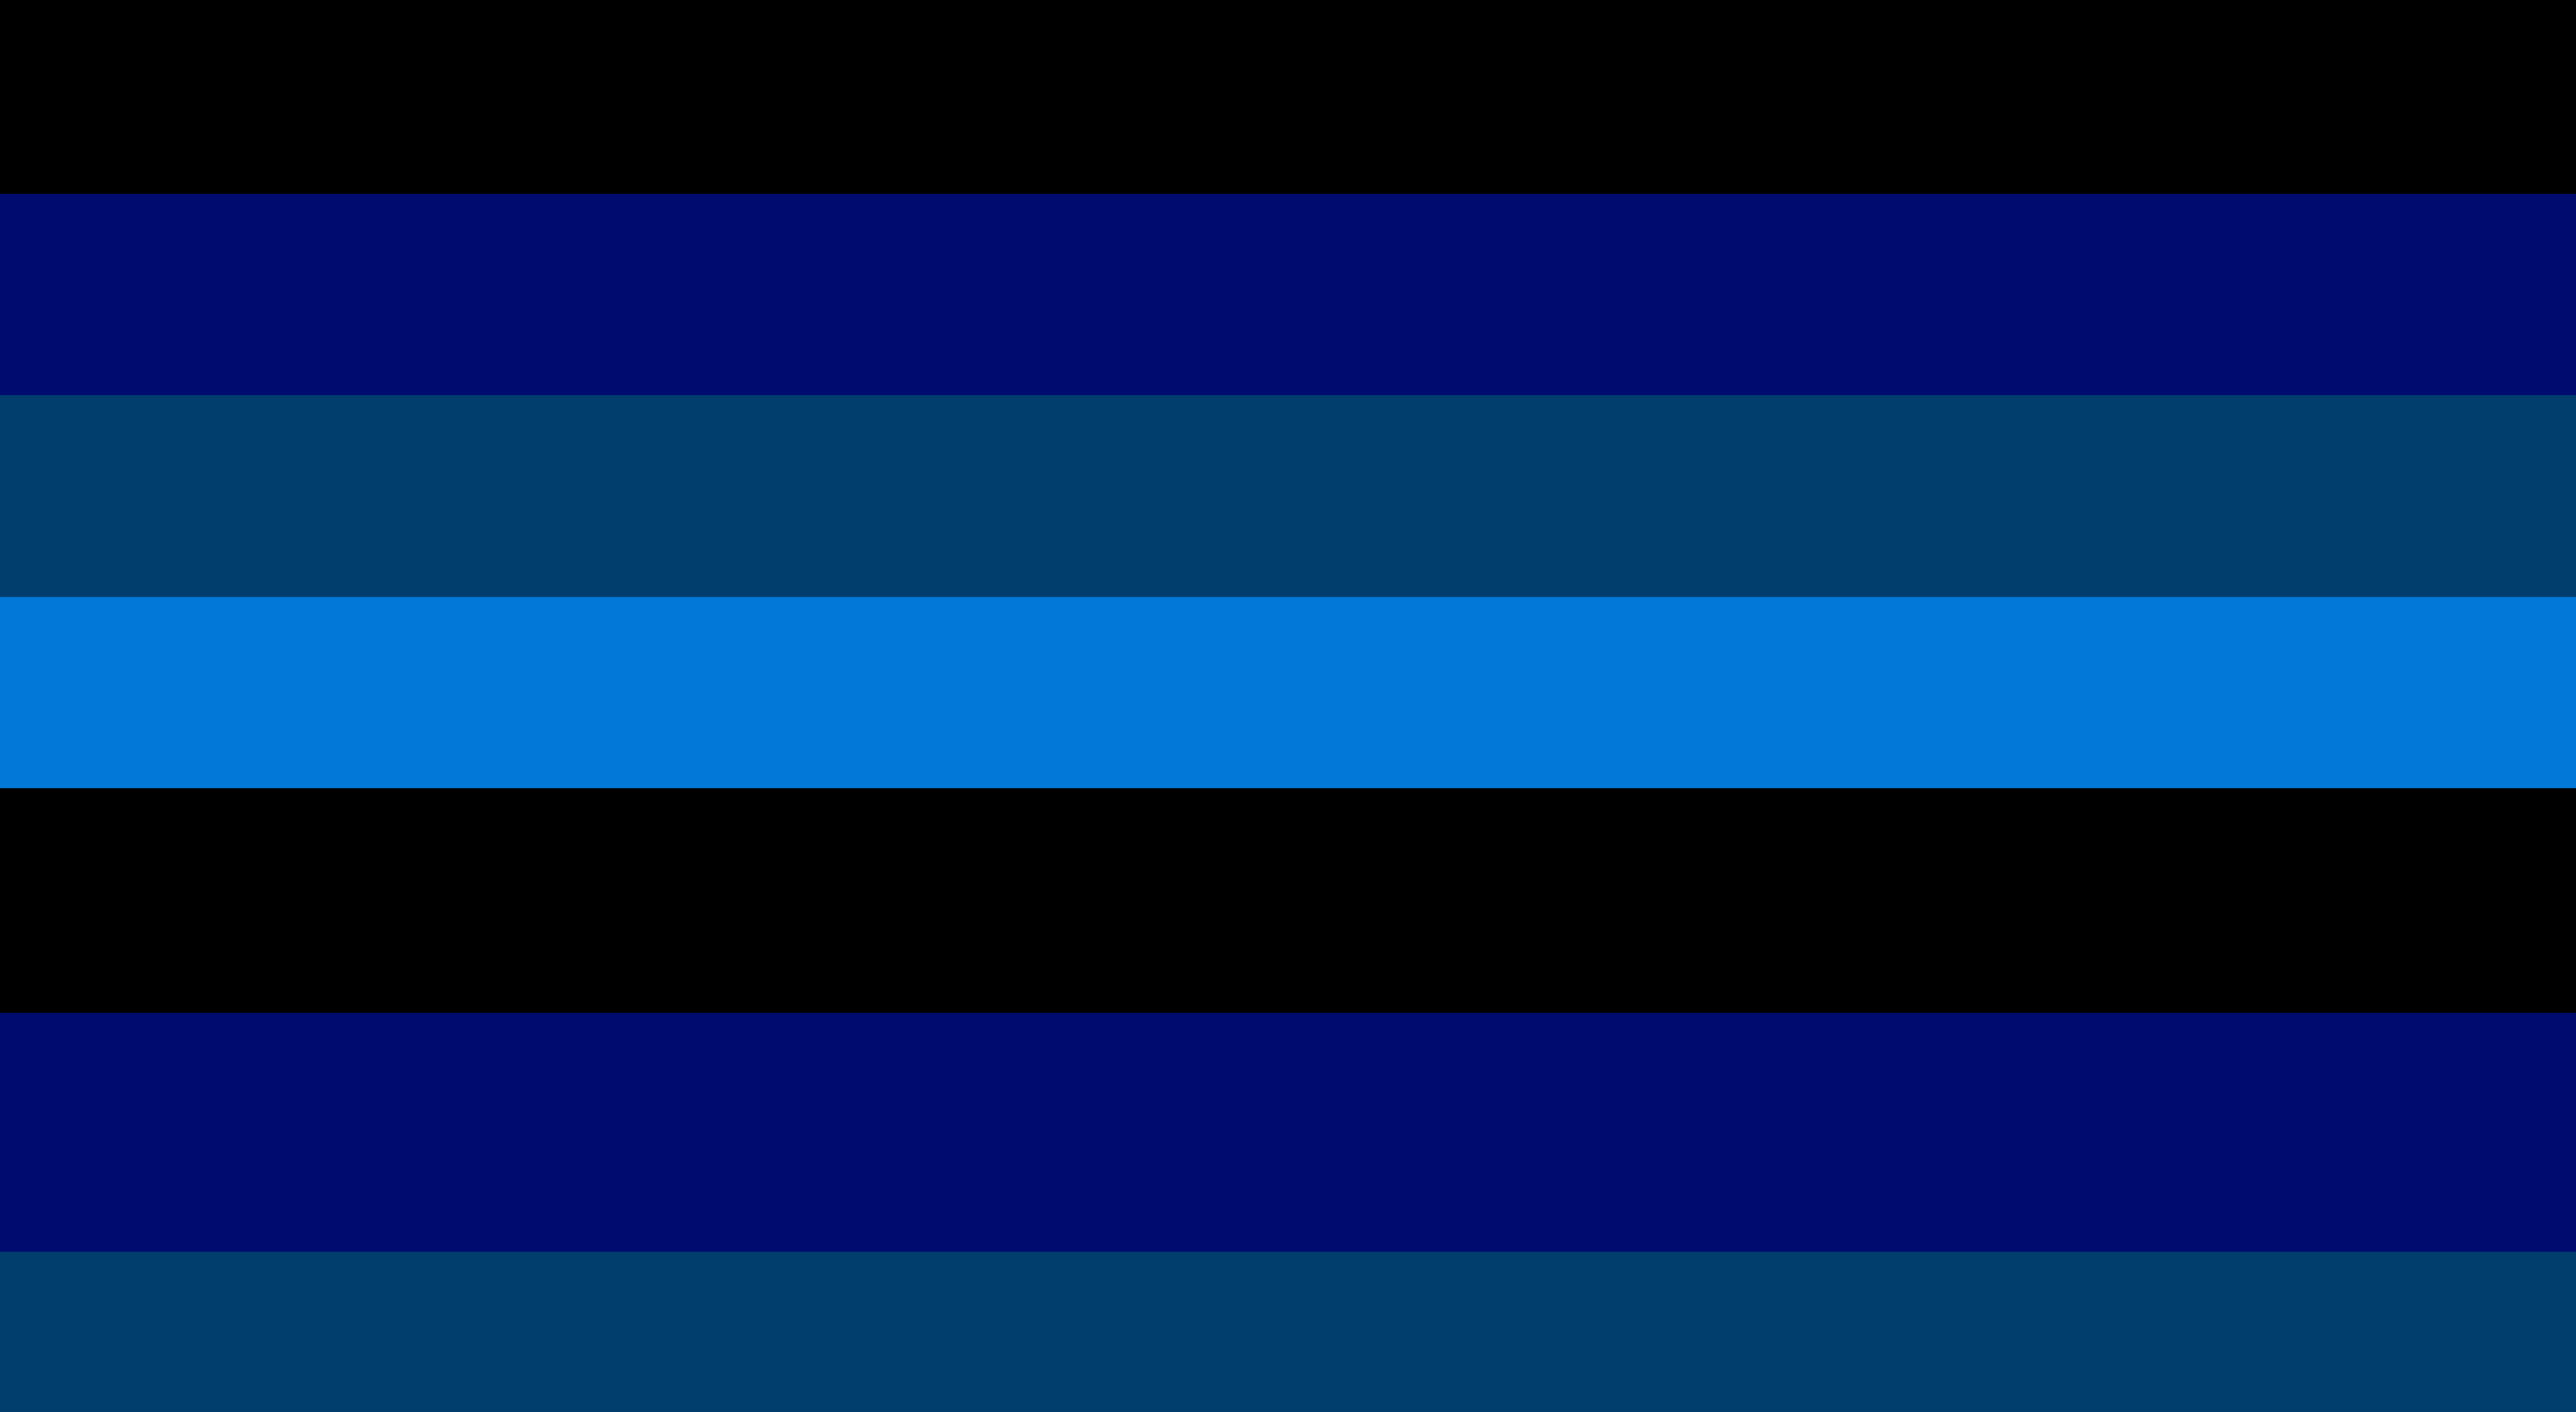
\includegraphics[width=4cm]{geo1.png}
  \setcaptionwidth{14cm}
  \caption{Geometry of the dieseFoam tutorial case.}
  \label{geo1}
\end{figure}
\newpage
\section{Pre-processing}
This section covers the necessary setup needed to get the dieselFoam case running with chemistry, the tutorial also covers a brief introduction to reacting flows in numerical simulations.

\subsection{Getting started}
Copy the dieselFoam tutorial to the run directory. 
\begin{verbatim}
cp -r  $FOAM_TUTORIALS/dieselFoam/aachenBomb $FOAM_RUN
cd $FOAM_RUN/aachenBomb
\end{verbatim}
The file structure of the dieselFoam case is similar to other OpenFOAM tutorials where the case directory has a \verb+/0+, \verb+/constant+ and \verb+/system+ directory. The dieselFoam case also has a \verb+/chemkin+ directory where the gas phase reaction schemes are specified. As usual in OpenFOAM tutorials; the solver-, write- and time-control can be found in the \verb+/system+ directory and the mesh setup in \verb+/constant/polyMesh+. 

\subsection{Boundary and initial conditions}
\label{Boundary and initial conditions}
Since there are neither outlets nor inlets, apart from the injector, the boundary conditions for the dieselFoam tutorial are very simple. All walls are modeled as adiabatic. 
The boundary conditions for the injector can be found in \verb+/constant/injectorProperties+ file see example below. 
\begin{verbatim}
        injectorType        unitInjector;

        unitInjectorProps
        {
            position        (0 0.0995 0);
            direction       (0 -1 0);
            diameter        0.00019;
            Cd              0.9;
            mass            6e-06;
            temperature     320;
            nParcels        5000;

            X
            (
                1.0
            ); 
	    massFlowRateProfile
            (
                (0 0.1272)
                (4.16667e-05 6.1634)
                (8.33333e-05 9.4778)
                ...
            );            		
\end{verbatim}
In the \verb+/constant/injectorProperties+ file it can be seen that the injector is located 0.5 mm from the top of the domain and injects in the negative y direction. Furthermore, the injector nozzle diameter, the nozzle discharge coefficient, mass and temperature of the parcels can be found here as well as the total number of injected parcels. The X is the mass fraction of a specific specie which will be described further in section \ref{Adding a second liquid to the the droplet}. The \verb+massFlowRateProfile+ specifies how the mass flow rate should vary over time. From time $t_0 \rightarrow t_1$ the mass flow rate is $\dot{m}_0$. This done in order to simulate opening and closing of the injector. The left column of the \verb+massFlowRateProfile+ is $t_i$ and the right, $\dot{m}_i$. 
\newpage
\noindent
It is possible to define different kinds of injectors, however, in this tutorial only the \verb+unitInjector+ will be used. In the \verb+/constant/sprayProperties+ file the user can specify what will happen to the droplets as they enter the domain, see table \ref{Model settings in /constant/sprayProperties-file for the dieselFoam tutorial}.  
\begin{table}[h]
\begin{center}
\begin{tabular}{l|l}
	Model & General meaning  \\ \hline
	subCycles & Minimum number of Lagrangian sub cycles\\
	atomizationModel & How atomization is treated \\
	includeOscillation & Droplet deformation; will effect droplet drag coefficient\\
	breakupModel & If secondary break up is used \\
	injectorModel & Which injector model to use \\
	collisionModel & Particle - particle interaction \\
	evaporationModel & Which evaporation model to use \\
	heatTransferModel & Particle heat transfer model \\
	dispersionModel & If turbulent dispersion is used or not \\
	dragModel &  Particle drag model\\
	wallModel & What happens to particles hitting the walls
\end{tabular}
\caption{Spray sub-models for the dieselFoam tutorial}
\label{Model settings in /constant/sprayProperties-file for the dieselFoam tutorial}
\end{center}
\end{table}
\newline
\noindent
The initial conditions are found in the \verb+/0+ directory and are summarized in table \ref{Initial conditions for the dieselFoam tutorial}. Not all initial conditions are specified here since they are not necessary to get the case running. Note that the initial mass fractions for $N_2$ and $O_2$ corresponds to air and that the initial condition for $spray$ is empty since it is specified in the \verb+/constant/injectorProperties+-file.    

\begin{table}[h]
\begin{center}
\begin{tabular}{l|l}
	Variable & Initial conditions  \\ \hline
	 $\epsilon$ 	& internalField       uniform 90.0,   		walls    	zeroGradient\\
	 $k$ 		& internalField       uniform 1.0,		walls		zeroGradient\\
	 $N_2$		& internalField       uniform 0.766, 		walls		zeroGradient\\
	 $O_2$		& internalField       uniform 0.233,  		walls		zeroGradient \\
	 $p$		& internalField       uniform 5e+06, 		walls		zeroGradient  \\
	 $spray$	& empty  \\
	 $T$		& internalField       uniform 800,  		walls		zeroGradient  \\
	 $U$		& internalField       uniform ( 0 0 0 ), 	walls		uniform ( 0 0 0 )  \\	  
\end{tabular}
\caption{Initial conditions for the dieselFoam tutorial}
\label{Initial conditions for the dieselFoam tutorial}
\end{center}
\end{table}
\newpage
\subsection{Physical properties}
In the \verb+/constant+ directory the properties files for chemistry, environment, spray, combustion, injector, RAS and thermophysical. The spray and injector properties are described in section \ref{Boundary and initial conditions} and the RAS properties are thoroughly described in the OpenFOAM user guide and are therefore not described here. The properties files are summarized in table \ref{Properties files and general content for the dieselFoam tutorial}.        

\begin{table}[h]
\begin{center}
\begin{tabular}{l|l}
	Properties file & General content \\ \hline
	chemistryProperties & Chemical reactions are included if \verb+chemistry+ is switched \verb+on+ \\ 
			    & Specification and settings for the discretization\\
			    & scheme used to solve the chemistry ODEs\\
	environmentalProperties & Gravity \\
	combustionProperties & Ignition point on or off, timing and duration of ignition point  \\
	thermophysicalProperties & Specify the mixture type and which gas phase reaction scheme \\ 
				 & to use as well as thermodynamic database
\end{tabular}
\caption{Properties files and general content for the dieselFoam tutorial}
\label{Properties files and general content for the dieselFoam tutorial}
\end{center}
\end{table}
\noindent
A certain mixture type may be more or less suited for a combustion problem and depends on if the flame is non-, partly or full-premixed. In the \verb+thermophysicalProperties+ file it is possible to specify the mixture types, several are available\footnote{http://www.opencfd.co.uk/openfoam/doc/thermophysicalModels.html}. Parts of the \verb+thermophysicalProperties+ file is listed below, notice that the location of the \verb+CHEMKINThermoFile+ has been changed from \verb+"~OpenFOAM/thermoData/therm.dat"+ to \verb+"$FOAM_CASE/chemkin/therm.dat"+. 
\begin{verbatim}
thermoType hMixtureThermo<reactingMixture>;
CHEMKINFile         "$FOAM_CASE/chemkin/chem.inp";
CHEMKINThermoFile   "$FOAM_CASE/chemkin/therm.dat";
\end{verbatim}
In this tutorial we will use the predefined \verb+reactingMixture+ together with the thermophysical model \verb+hMixtureThermo+ which calculates enthalpy for combustion mixture. The choice of mixture and thermo physical model depends both on the physics of the flame and which variables that are needed for the combustion model. The \verb+thermophysicalProperties+ file also contains information on where the gas phase reactions are defined as well which thermo dynamic data base to use. The gas phase reactions are specified in the \verb+"$FOAM_CASE/chemkin/chem.inp"+ file and the thermo dynamic data base in the \verb+"$FOAM_CASE/chemkin/therm.dat"+ file. The \verb+therm.dat+ and \verb+chem.inp+-file will be described further in section \ref{Chemistry} as well as the combustion model.    

\subsection{Chemistry}
\label{Chemistry}
When the droplets enter the domain they start to evaporate. The $C_7H_{16} (g)$ \footnote{Notation $(g)$  meaning that the specie is in gas phase. Similar notation is $(s)$ for solid and $(l)$ for liquid. The notation is used here to emphasize that no heterogeneous reactions are taking place.} then reacts with oxygen forming $CO_2$ and $H_{2}O$. However, this reaction can be called a global reaction and is not what would happen if $C_7H_{16} (g)$ would burn with air in a real combustor or burner. As an example, think about hydrogen burning with pure oxygen, see reaction \ref{H2O+O2}.  

\begin{equation}
\label{H2O+O2}
H_{2} +\frac{1}{2}O_{2} \Leftrightarrow H_{2}O	
\end{equation}    
\noindent
However, in order for the hydrogen to react with oxygen, the bond between the atoms first have to be broken and a more complex reaction scheme is required, see reaction \ref{H2+2H} to \ref{OH+H}.    

\begin{equation}
\label{H2+2H}
H_{2}  \Leftrightarrow 2H	
\end{equation}

\begin{equation}
\label{O2+2O}
O_{2}  \Leftrightarrow 2O	
\end{equation}

\begin{equation}
\label{H+O}
H+O  \Leftrightarrow OH	
\end{equation}

\begin{equation}
\label{OH+H_{2}}
OH+H_{2} \Leftrightarrow H_{2}O+H
\end{equation}

\begin{equation}
\label{OH+H}
OH+H \Leftrightarrow H_{2}O
\end{equation}

\noindent
So, instead of having two reactions (backward and forward) with three species we have ten reactions (backward and forward) with six species (the scheme described above is \textit{ad hoc} and is just used to describe the difficulties describing chemistry in numerical simulations). The transport equations for these species have to be solved as well as the ODEs for the reactions. 
\noindent
In this tutorial the gas phase reactions are specified in the \verb+/chemkin/chem.inp+-file, see below. 
\begin{verbatim}
REACTIONS
 C7H16 + 11O2            => 7CO2 + 8H2O        5.00E+8  0.0   15780.0! 1
        FORD    / C7H16 0.25 /
        FORD    / O2 1.5 /
END
\end{verbatim}
The entries behind the reaction in the  \verb+/chemkin/chem.inp+-file are Arrhenius coefficient that are used to calculate the chemical reaction rate. \verb+FORD+ is the forward reaction order. The chemical reaction rate will be calculated according to equations \ref{forward reaction coeff} and \ref{reaction rate }
\begin{equation}
\label{forward reaction coeff}
k_{f} = A  T^{b} \cdot exp \left(\frac{-E_{a}}{RT}\right) 	
\end{equation}
Where $k_{f}$ is the forward reaction coefficient, $A$ pre exponential factor, $b$ temperature exponent, $E_a$ activation energy, $R$ ideal gas coefficient and $T$ temperature.    
\begin{equation}
\label{reaction rate }
\dot{\omega_i}=\frac{ \text{d}   [product]}{\text{d}t}= -k_{f} * [fuel]^{c}  [oxidizer]^{d}
\end{equation}  
Where $\dot{\omega_i}$ is the chemical reaction rate, $t$  time, $c$ and $d$ the forward reaction order and, $[ C ]$ is concentration of specie $C$. In simplified terms the \verb+/chemkin/chem.inp+-file can thus be written as:
\begin{verbatim}
REACTIONS
 fuel + oxidizer            => product        A  b  Ea 
        FORD    / fuel c /
        FORD    / oxidizer d /
END
\end{verbatim} 
\noindent
Due to the numerical cost only the simplest scheme (chem.inp) will be used in this tutorial but the user is encouraged to look in the chem.inp.full file to see how a complex but still reduced reaction scheme might look like.
\newline 
\newline
\noindent
With out going into great detail regarding thermodynamics in combustion processes\footnote{Combustion 4th edition, Chapter 4, J.Warnatz et al. Springer 2006}, it is possible to realize that when a fuel and an oxidizer react, they will produce heat. The amount of heat released from the flame as well as the flame temperature can be predicted using thermodynamics. The thermodynamic data base is located in the  \verb+/chemkin/therm.dat+-file. An example from the \verb+/chemkin/therm.dat+-file is listed below.  
\begin{verbatim}
C7H16             P10/95 C   7H  16    0    0G   200.000  5000.000  1391.000    1
 2.22148969e+01 3.47675750e-02-1.18407129e-05 1.83298478e-09-1.06130266e-13     2
-3.42760081e+04-9.23040196e+01-1.26836187e+00 8.54355820e-02-5.25346786e-05     3
 1.62945721e-08-2.02394925e-12-2.56586565e+04 3.53732912e+01                    4
\end{verbatim}
\begin{itemize}
\item The first row contains species name, date (not used in the code), atomic symbols and formula, phase of species (S, L, or G for gas), low temperature, high temperature and common temperature (if needed).
\item The second row contains coefficients $a_{1}-a_{5}$ in equation \ref{Cp} for upper temperature interval.
\item The third row contains coefficients $a_{6}$, $a_{7}$ for upper temperature interval, and $a_{1}$, $a_{2}$, and $a_{3}$ for lower.

\item The fourth row contains coefficients $a_{4}$, $a_{5}$, $a_{6}$, $a_{7}$ for lower temperature interval.
\end{itemize}
From these constants, (NASA) polynomials for specific heat $C_{p}$, enthalpy $H$ and entropy $S$ can be calculated.
\begin{equation}
\label{Cp}
 	\frac{C_{p}} {R} = a_{1}+a_{2} \cdot T +a_{3} \cdot T^{2}+a_{4} \cdot T^{3}+a_{5} \cdot T^{4}
\end{equation} 

\begin{equation}
\label{H}
 	\frac{H}{RT} = a_1 + \frac{a_2 T}{2} + \frac{a_3 T^2} {3} + \frac{a_4 T^3}{4} + \frac{a_5 T^4}{5} + \frac{a_6}{T}
\end{equation} 

\begin{equation}
\label{S}
 \frac{S}{R}  = a_1 \text{ln}T + a_{2} T + \frac{a_{3} T^2}{2} + \frac{a_4 T^3 }{3} + \frac{a_5 T^4}{4} + a_7
\end{equation}
The specific heat $C_{p}$, enthalpy $H$ and entropy $S$ are then used in the code to solve the conservation equations.
\newline
\newline
\noindent
The combustion model for this tutorial is a partially stirred reactor concept model developed at Chalmers Gothenburg described by equations \ref{CST} and \ref{tau_{mix}}
\begin{equation}
\label{CST}
	CST_{i}=\frac{\tau_{chem}}{\tau_{mix}+\tau_{chem}}\dot{\omega_i}
\end{equation}
Where $CST_{i}$ is the chemical source term, $\tau_{chem}$ chemical time $\propto \frac{1}{k_{f}}$ and $\tau_{mix}$ mixing time.
The mixing time $\tau_{mix}$ is calculated according to 
\begin{equation}
\label{tau_{mix}}
	\tau_{mix}= C_{mix}\sqrt{\frac{\mu_{eff}}{\rho  \epsilon}}.
\end{equation}
Where $C_{mix}$ is a constant specified in the \verb+/constant/combustionProperties+-file,  $\mu_{eff}$ is the effective viscosity, $\rho$ density and $\epsilon$ rate of dissipation of turbulent kinetic energy. The combustion model can be found on lines 81-95 in \verb+$FOAM_SOLVERS/combustion/dieselFoam/dieselFoam.C+


\section{Running the code}
Remove \verb+ft+ and \verb+fu+ and in the \verb+aachenBomb/0+ directory since these are not needed for this setup (keeping them will result in post-processing problems).  
\begin{verbatim}
cd $FOAM_RUN/aachenBomb/0
rm ft fu 
\end{verbatim} 
Turn chemistry on in the \verb+/constant/chemistryProperties+ file
\begin{verbatim}
chemistry               on;
\end{verbatim} 
\noindent
and ignition on in the \verb+/constant/combustionProperties+  file. This step is not necessary, the mixture will still ignite when the species are properly mixed due to the high temperature. 
\begin{verbatim}
ignite              	on;
\end{verbatim} 
Mesh the geometry using \verb+blockMesh+, and start the \verb+dieselFoam+ solver.
\begin{verbatim}
cd $FOAM_RUN/aachenBomb
blockMesh
dieselFoam              	
\end{verbatim} 
The solution is only 0.01 seconds long, however, due to the fast chemistry a minimum of 4000 time steps are needed to resolve it. Furthermore, there is a total of 5000 parcels ($parcel_{mass} = N*Droplet_{mass}$ where $N$ is the statistical number of drops in the parcel) that enter the domain and the source term from these all have to be calculated.  
\section{Post-processing in ParaView}
\label{Post-processing in ParaView}
Since paraFoam can not handle Lagrangian particles use foamToVTK and then ParaView.
\begin{verbatim}

cd $FOAM_RUN/aachenBomb
foamToVTK  
paraview          	
\end{verbatim} 
In the /VTK directory open the case file ( \verb+aachenBomb\1.vtk+ ) and also, open the particles in the \verb+/Lagrangian/defaultCloud_2.vtk+ file.
Create glyphs for the particles, see figure \ref{Settings for glyphs in ParaView to visualize the Lagrangian particles} for settings.

\begin{figure}[h]
\begin{center}
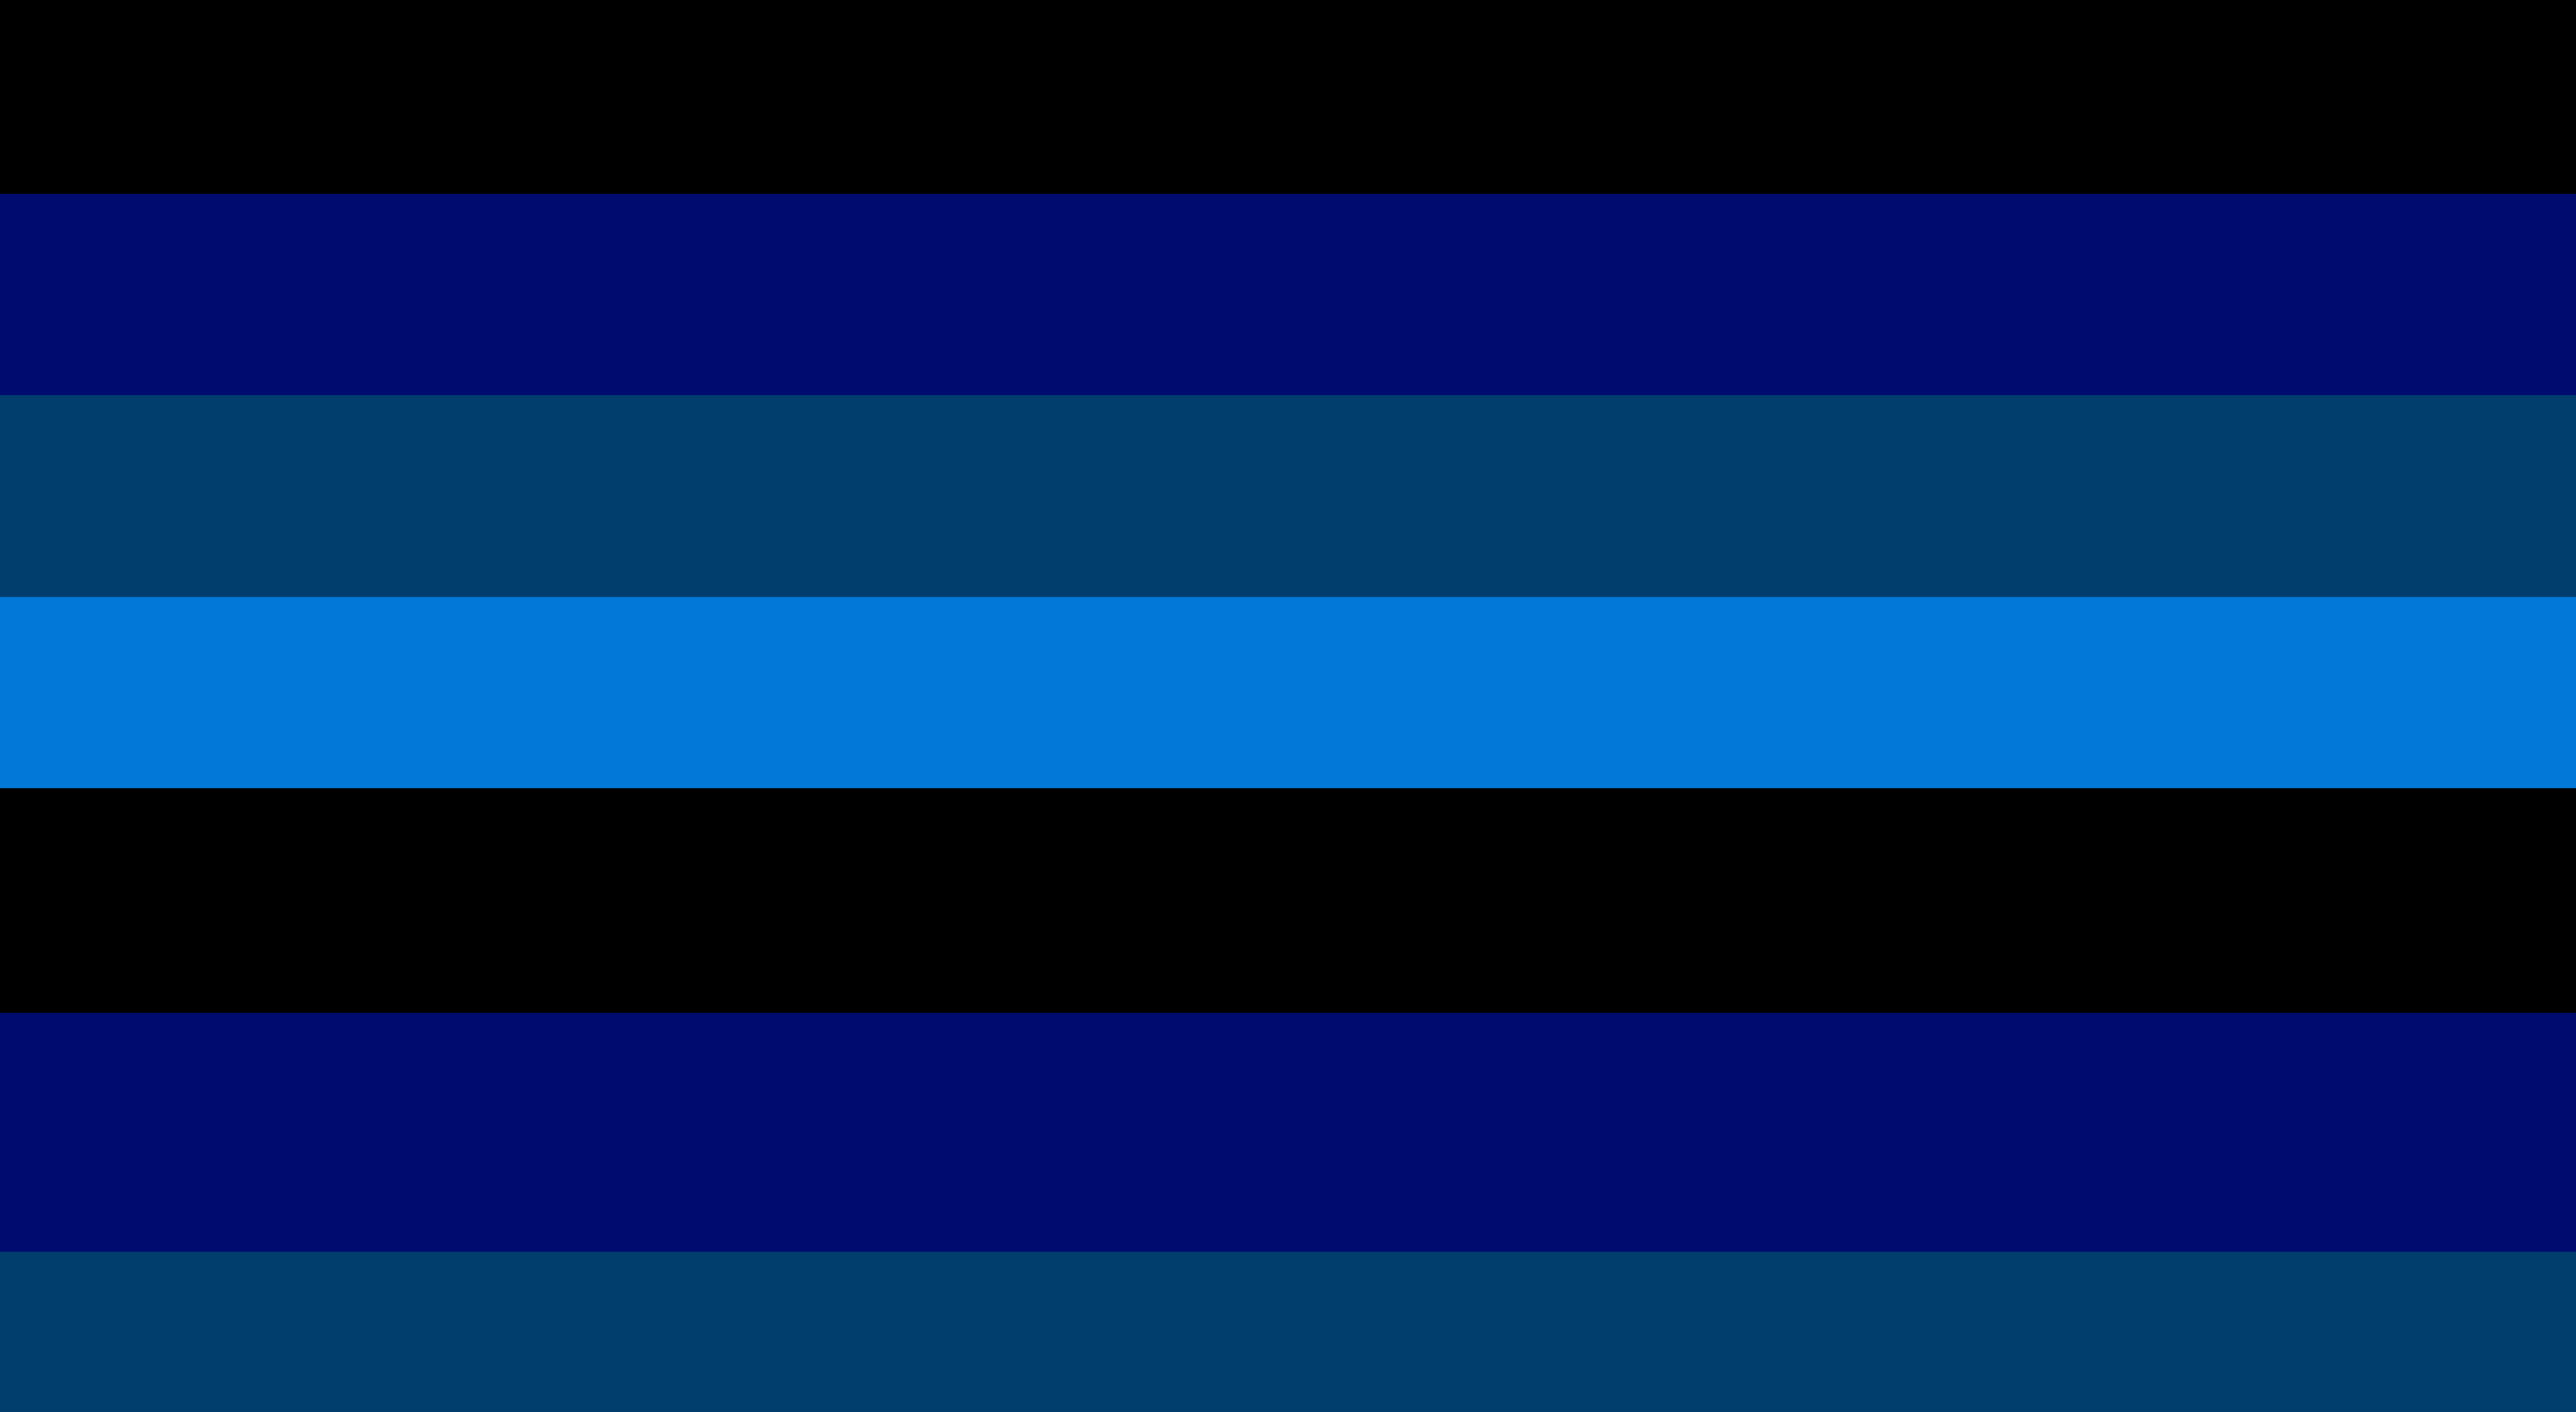
\includegraphics[width=5cm]{glyphs_paraview.png}
\end{center}
\caption{Settings for glyphs in ParaView to visualize the Lagrangian particles}
\label{Settings for glyphs in ParaView to visualize the Lagrangian particles}
\end{figure}
\newpage


\begin{figure}[ht]
\begin{center}
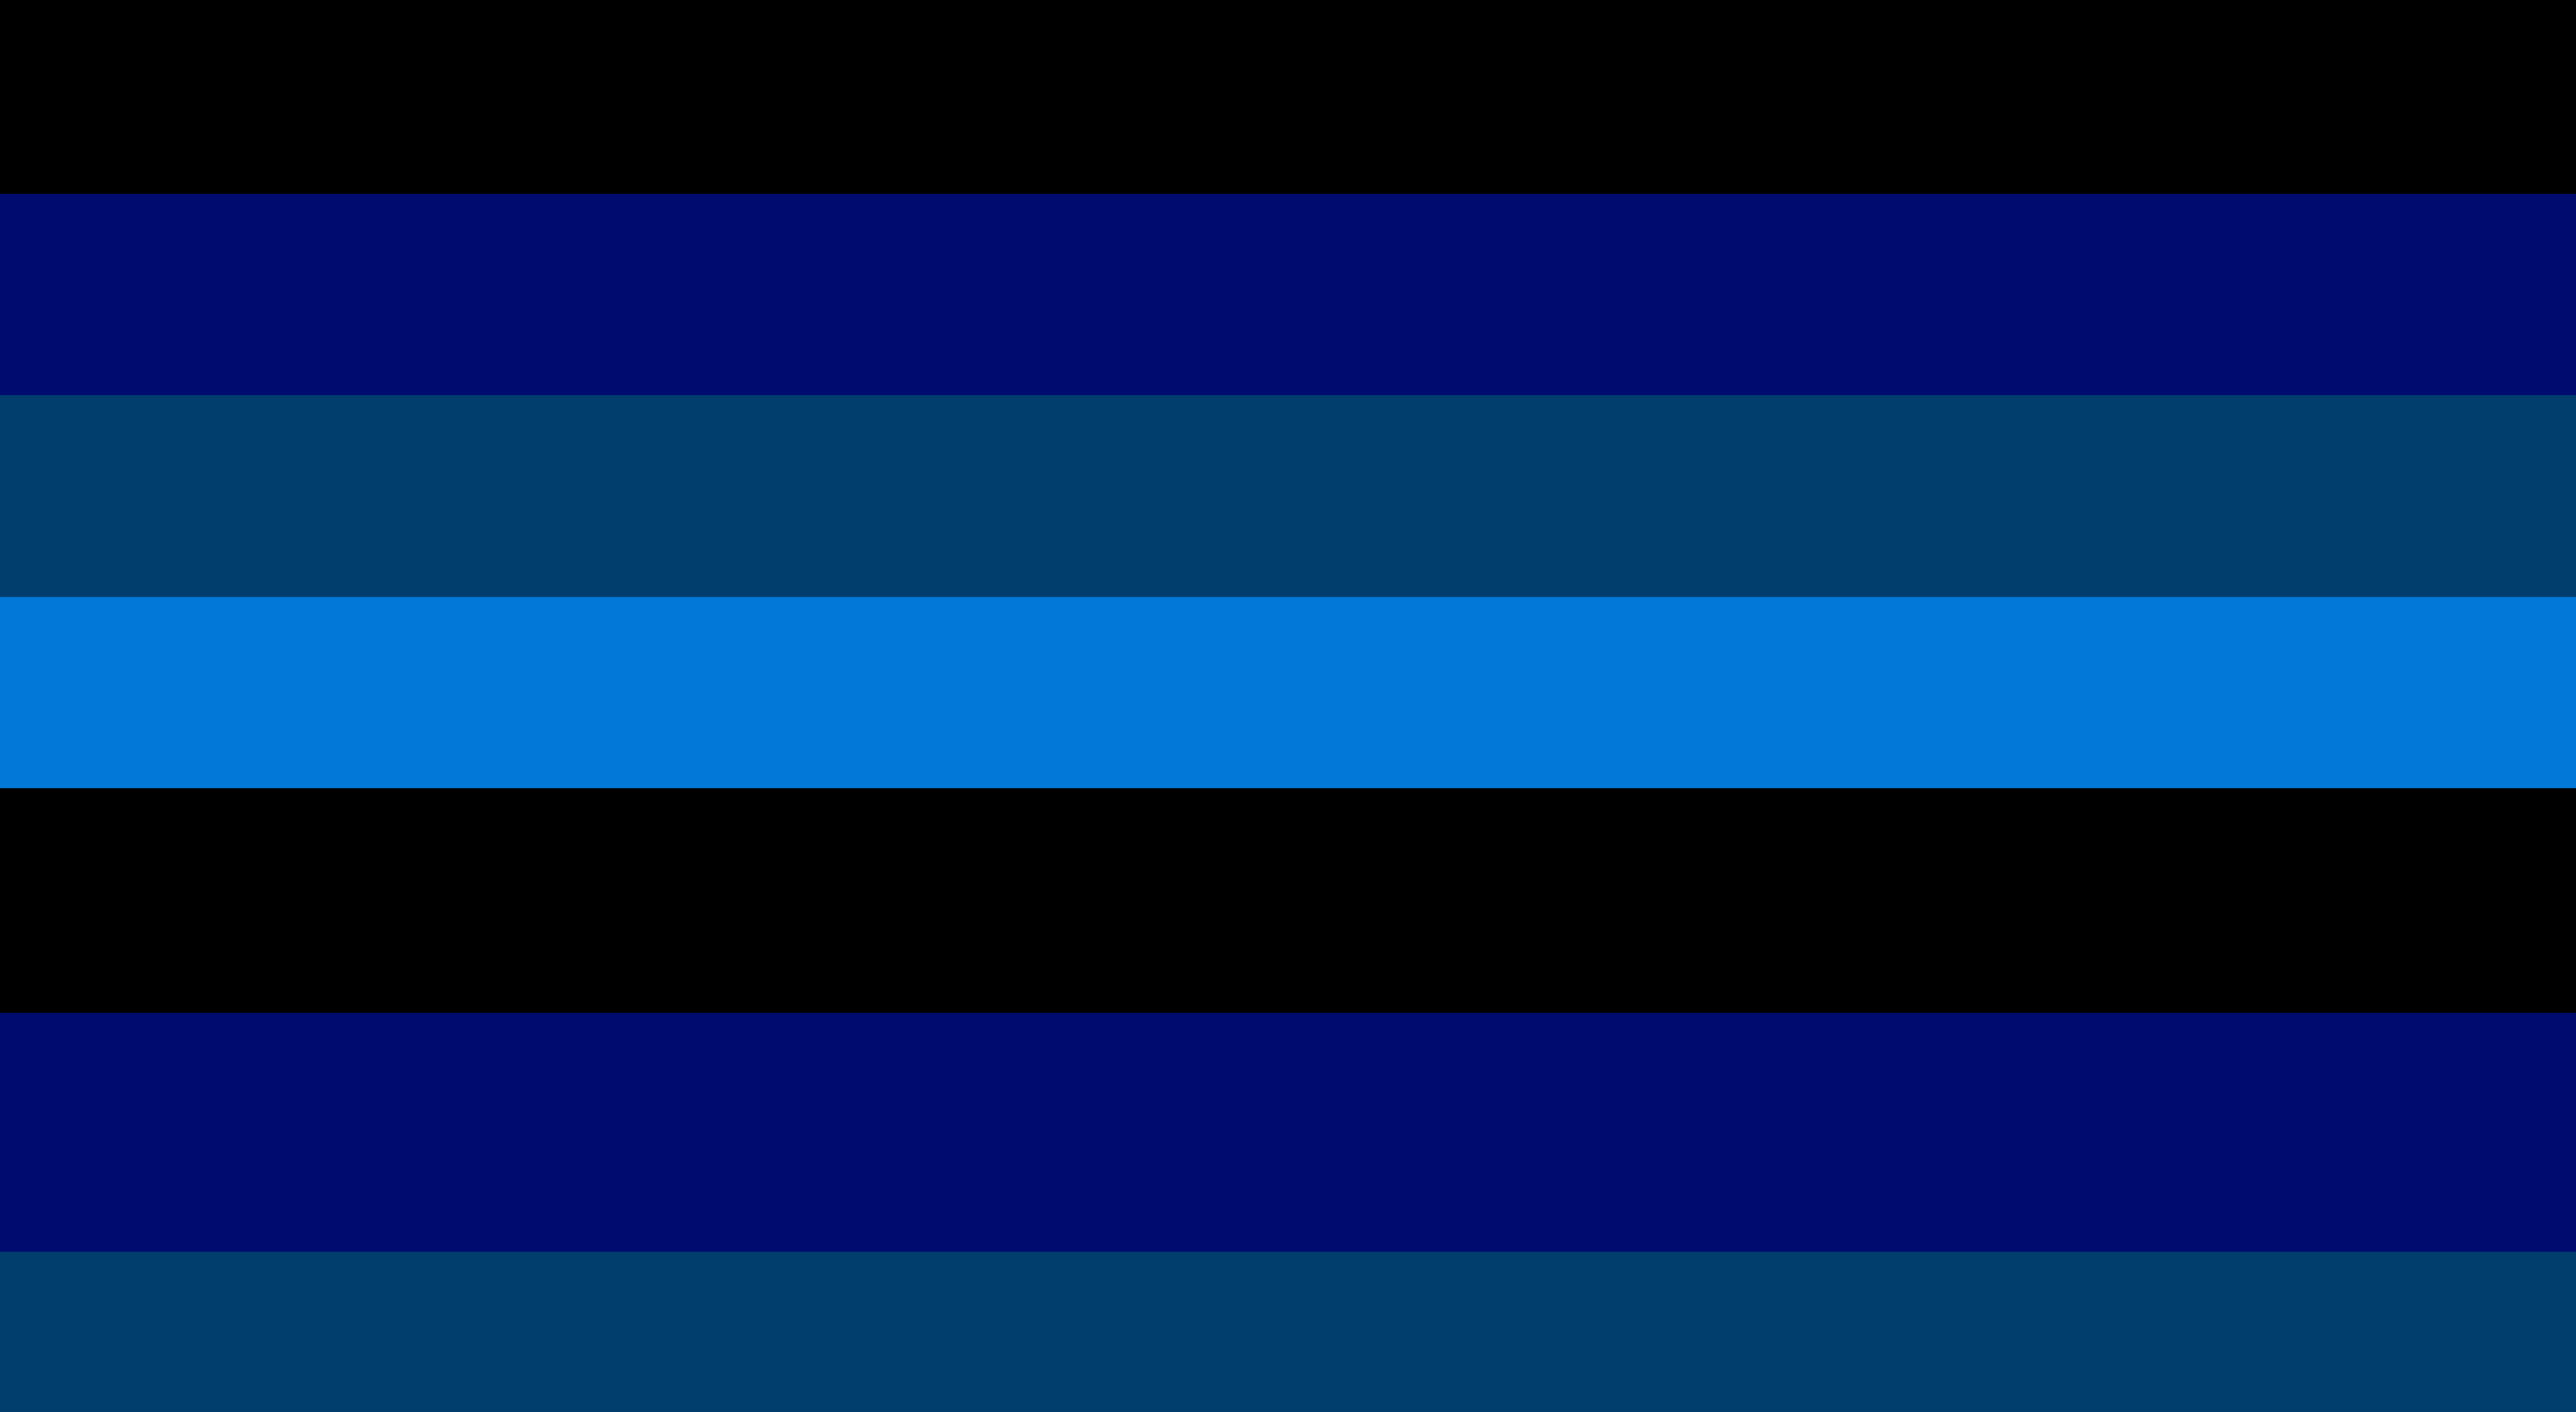
\includegraphics[width=10cm]{drops_and_diamter_8.png}
\end{center}
\caption{Droplets entering the domain, droplets colored by diameter and cut plane by temperature}
\label{Droplets entering the domain, droplets colored by diameter and cut plane by temperature}
\end{figure}

\begin{figure}[ht]
\begin{center}
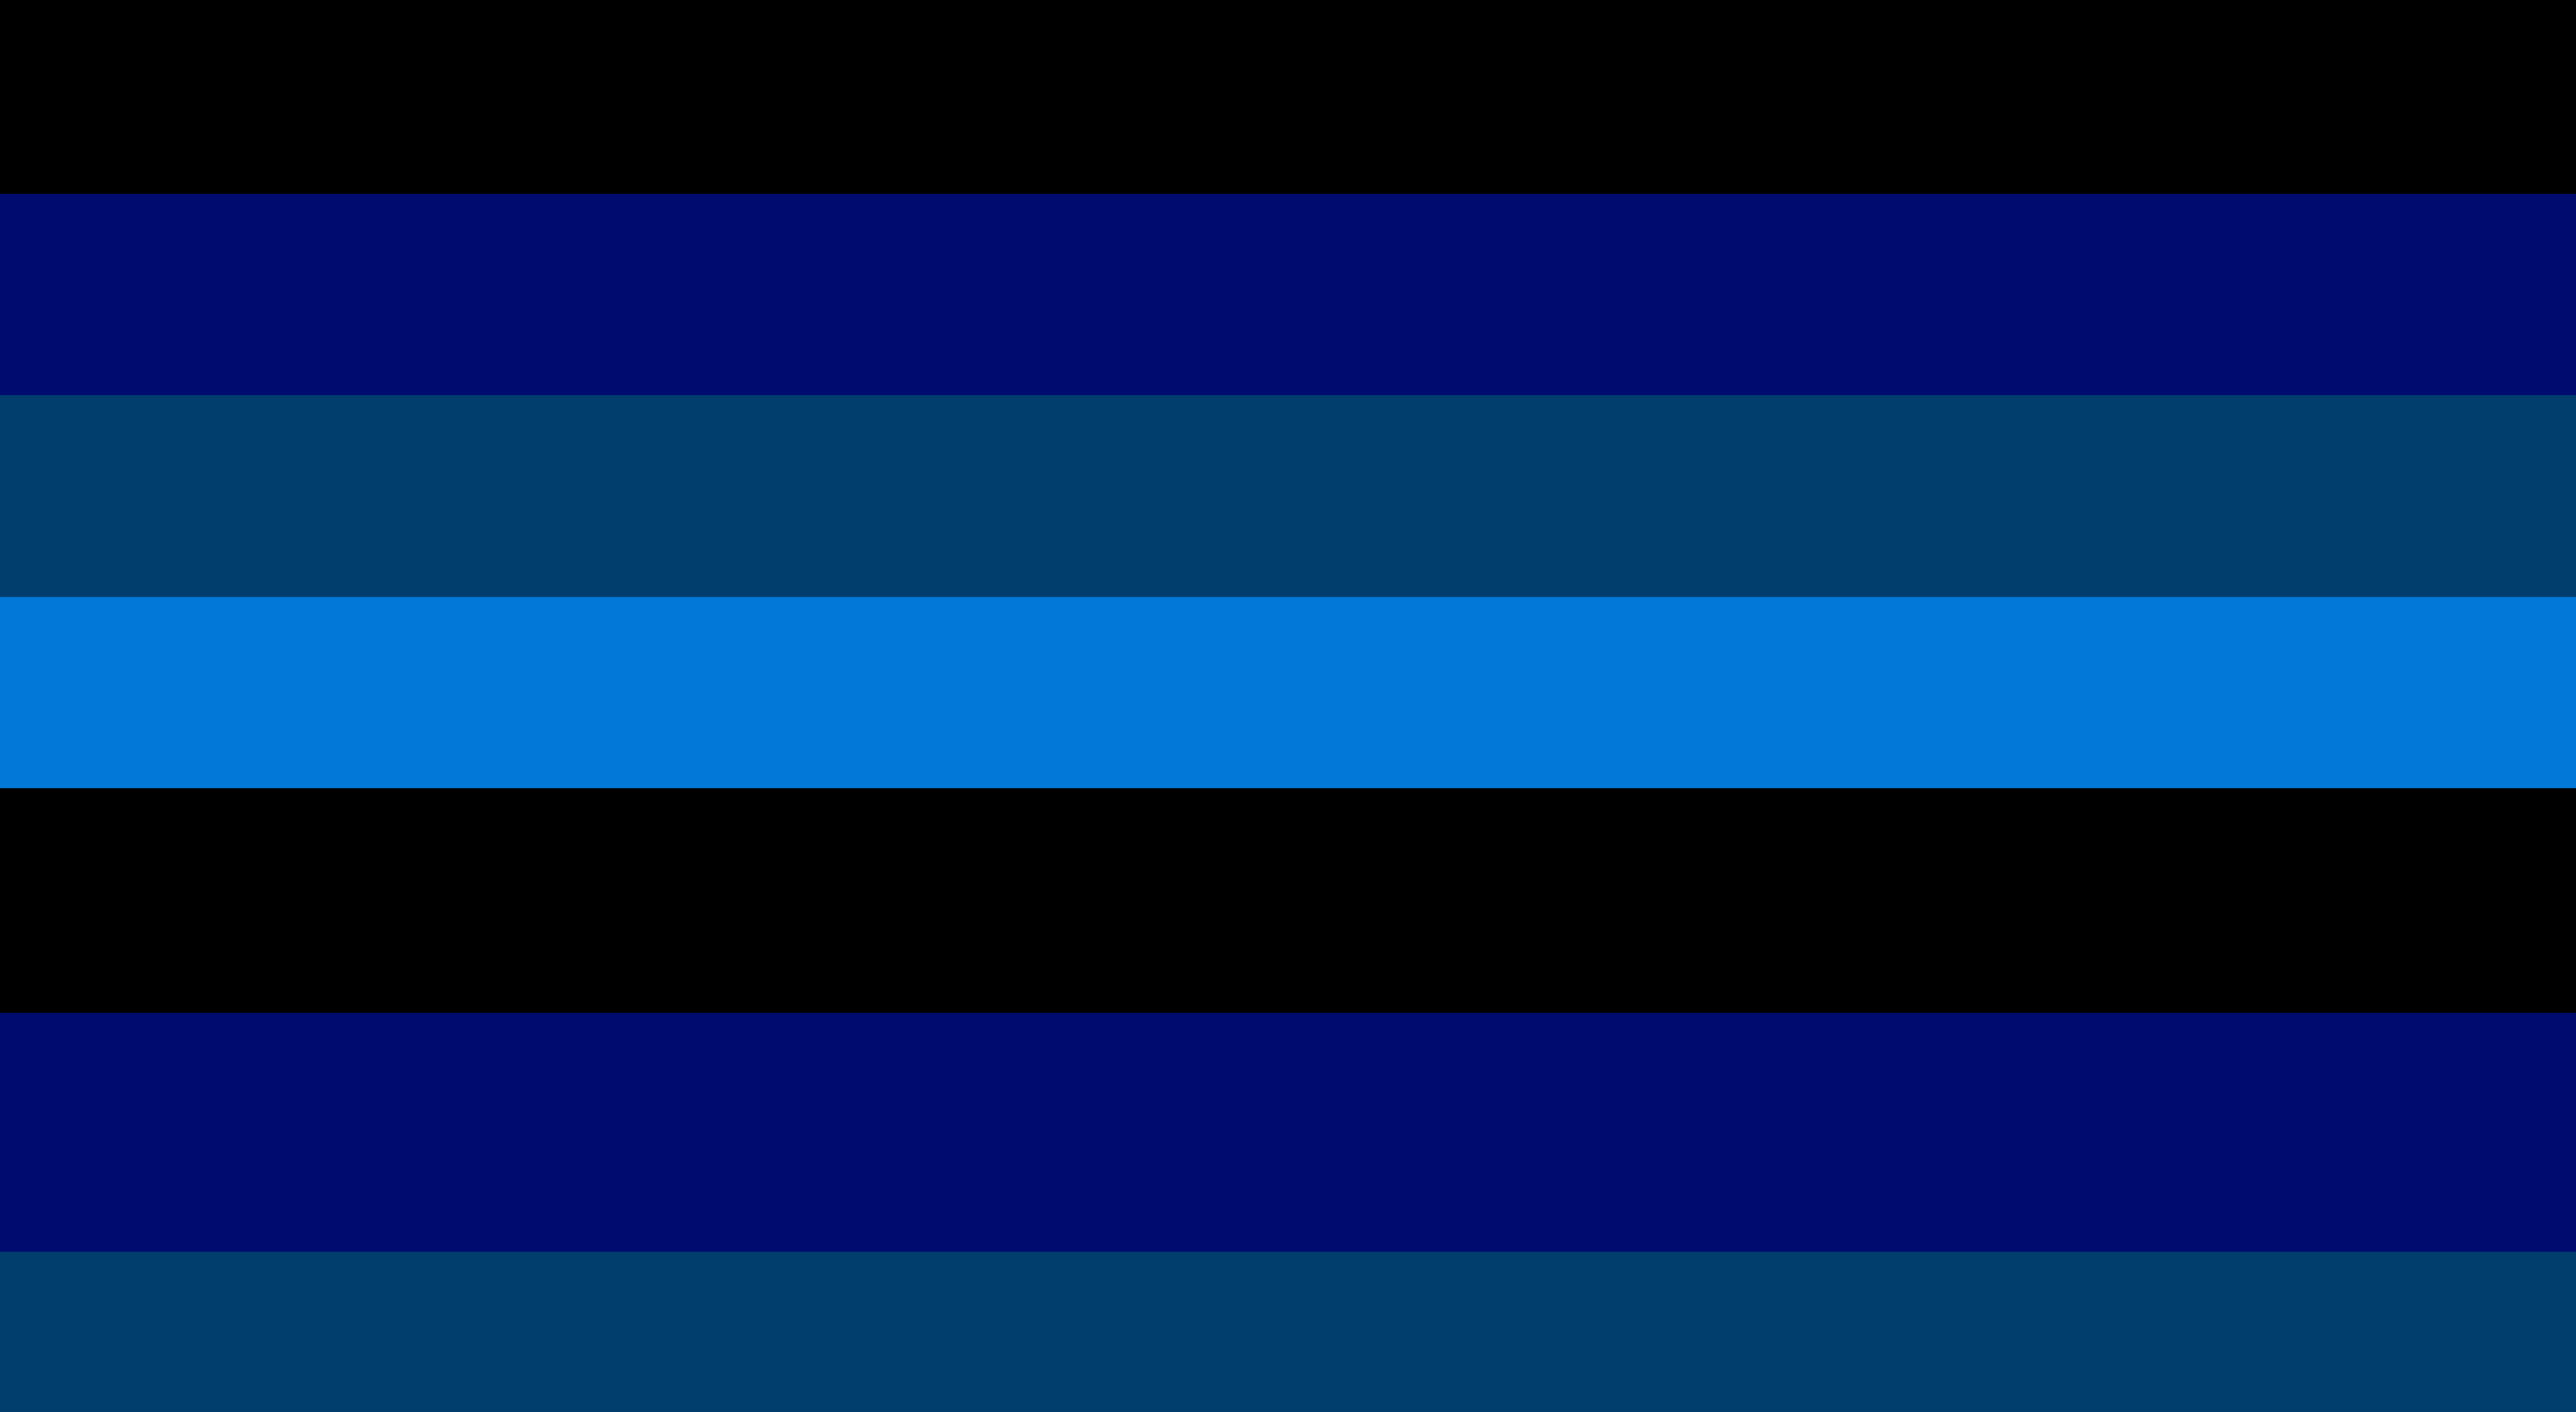
\includegraphics[width=10cm]{ignition.png}
\end{center}
\caption{Gas phase ignition, droplets colored by diameter and cut plane by temperature}
\label{Gas phase ignition, droplets colored by diameter and cut plane by temperature}
\end{figure}

\newpage
\section{Adding a second liquid}
\label{Adding a second liquid to the the droplet}
To add a second liquid to the droplets follow these step-by-step instructions.\newline
\newline
\noindent
Remove \verb+ft+ and \verb+fu+  in the \verb+aachenBomb/0+ directory  since these are not needed for this setup.
\begin{verbatim}
cd $FOAM_RUN/aachenBomb/0
rm ft fu 
\end{verbatim} 
Turn chemistry on in the \verb+/constant/chemistryProperties+ file

\begin{verbatim}
chemistry               on;
\end{verbatim} 

\noindent
and ignition on in the \verb+/constant/combustionProperties+  file.

\begin{verbatim}
ignite              	on;
\end{verbatim} 

\noindent
In \verb+aachenBomb/constant/thermophysicalProperties+ add an extra liquid material, here $C_{6}H_{14}$ is used as an example. 
\begin{verbatim}
liquidComponents
(
    C7H16
    C6H14
);

liquidProperties
{
    C7H16  C7H16 defaultCoeffs;
    C6H14  C6H14 defaultCoeffs;
}
\end{verbatim}
In \verb+aachenBomb/chemkin/chem.inp+ add the $C_{6}H_{14}$ in species.
\begin{verbatim}
ELEMENTS
 H   O    C   N   AR
END
SPECIE
C6H14 C7H16 O2 N2 CO2 H2O
END
REACTIONS
 C7H16 + 11O2            => 7CO2 + 8H2O        5.00E+8  0.0   15780.0! 1
        FORD    / C7H16 0.25 /
        FORD    / O2 1.5 /
END
\end{verbatim}

\noindent 
In \verb+aachenBomb/constant/injectorProperties+ change the mass fractions for $C_{7}H_{16}$ and $C_{6}H_{14}$.
\begin{verbatim}
 X
            (
                0.8
                0.2
            );
\end{verbatim}
The droplets will now consist of 80 weight percent $C_{7}H_{16}$ and 20 percent $C{6}H_{14}$. Mesh the geometry using \verb+blockMesh+, and start the \verb+dieselFoam+ solver.
\begin{verbatim}
cd $FOAM_RUN/aachenBomb
blockMesh
dieselFoam              	
\end{verbatim} 
\noindent
Post in ParaView as described in section \ref{Post-processing in ParaView}. Notice the difference in evaporation pressure between the two species $C_{6}H_{14}$ and $C_{7}H_{16}$.

\begin{figure}[h]
  \centering
  \subfloat[$C_{6}H_{14}$]{\label{fig:gull}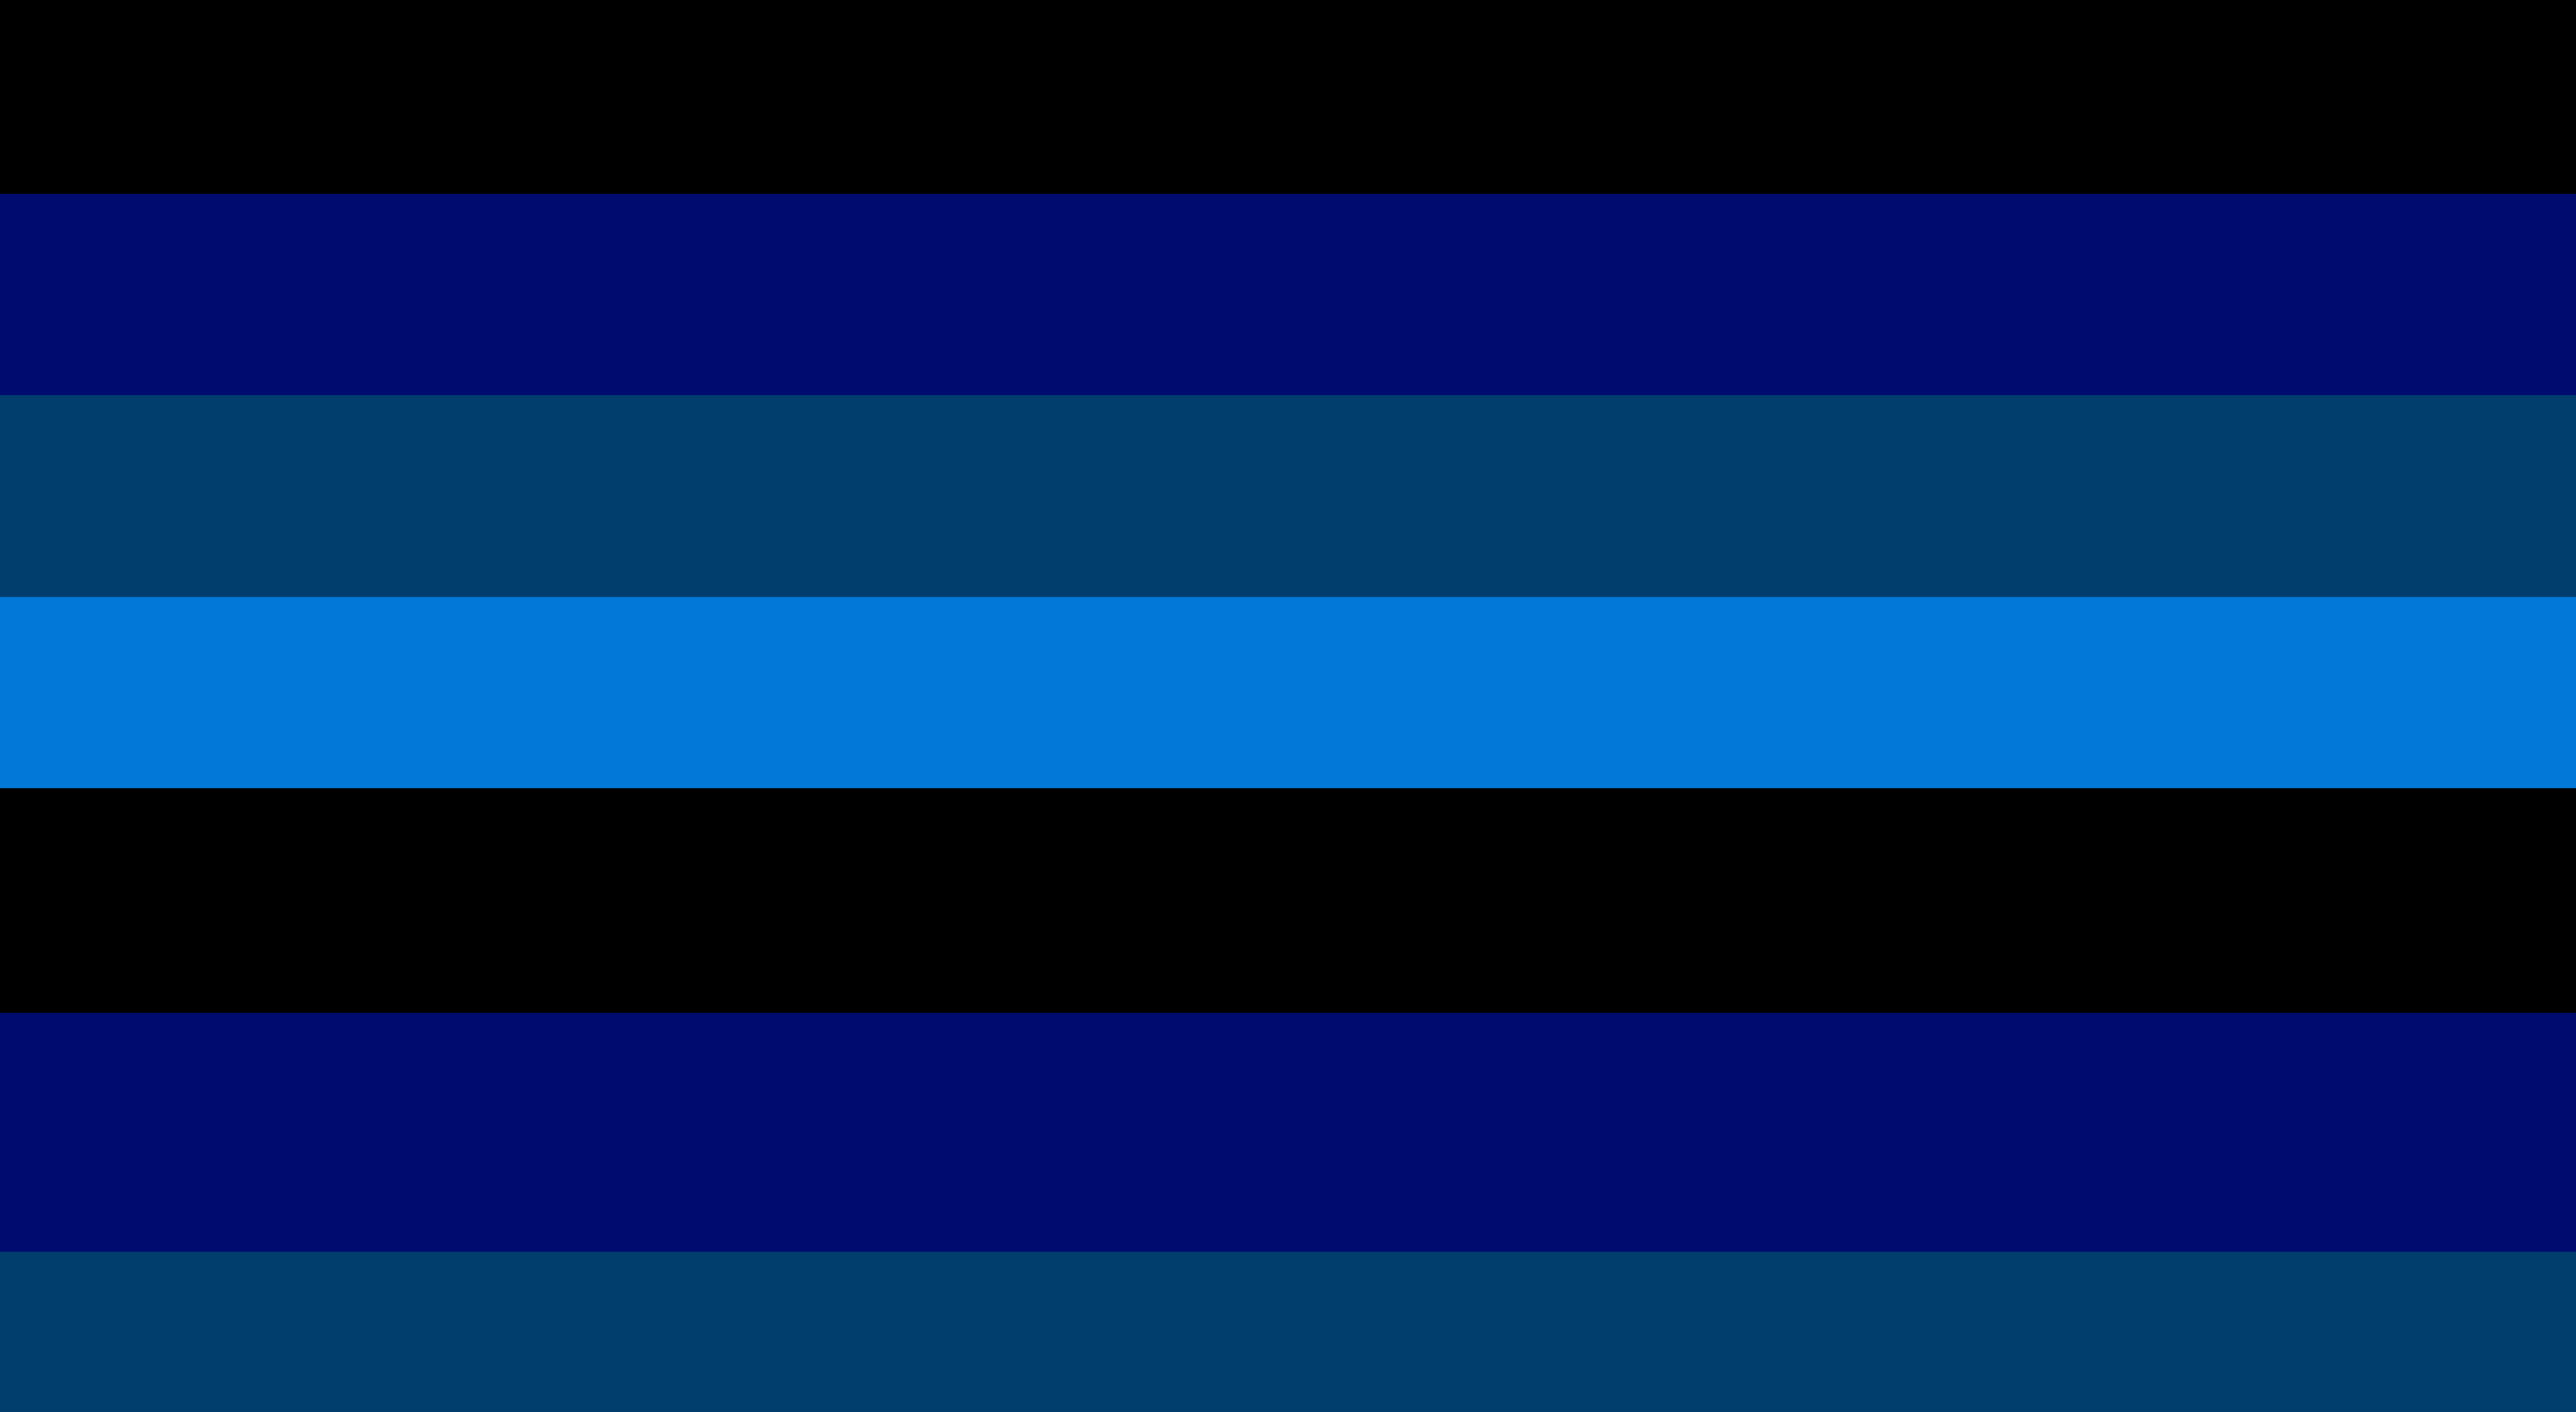
\includegraphics[width=0.3\textwidth]{C6H14.png}}
	\hspace{1in}               
  \subfloat[$C_{7}H_{16}$]{\label{fig:tiger}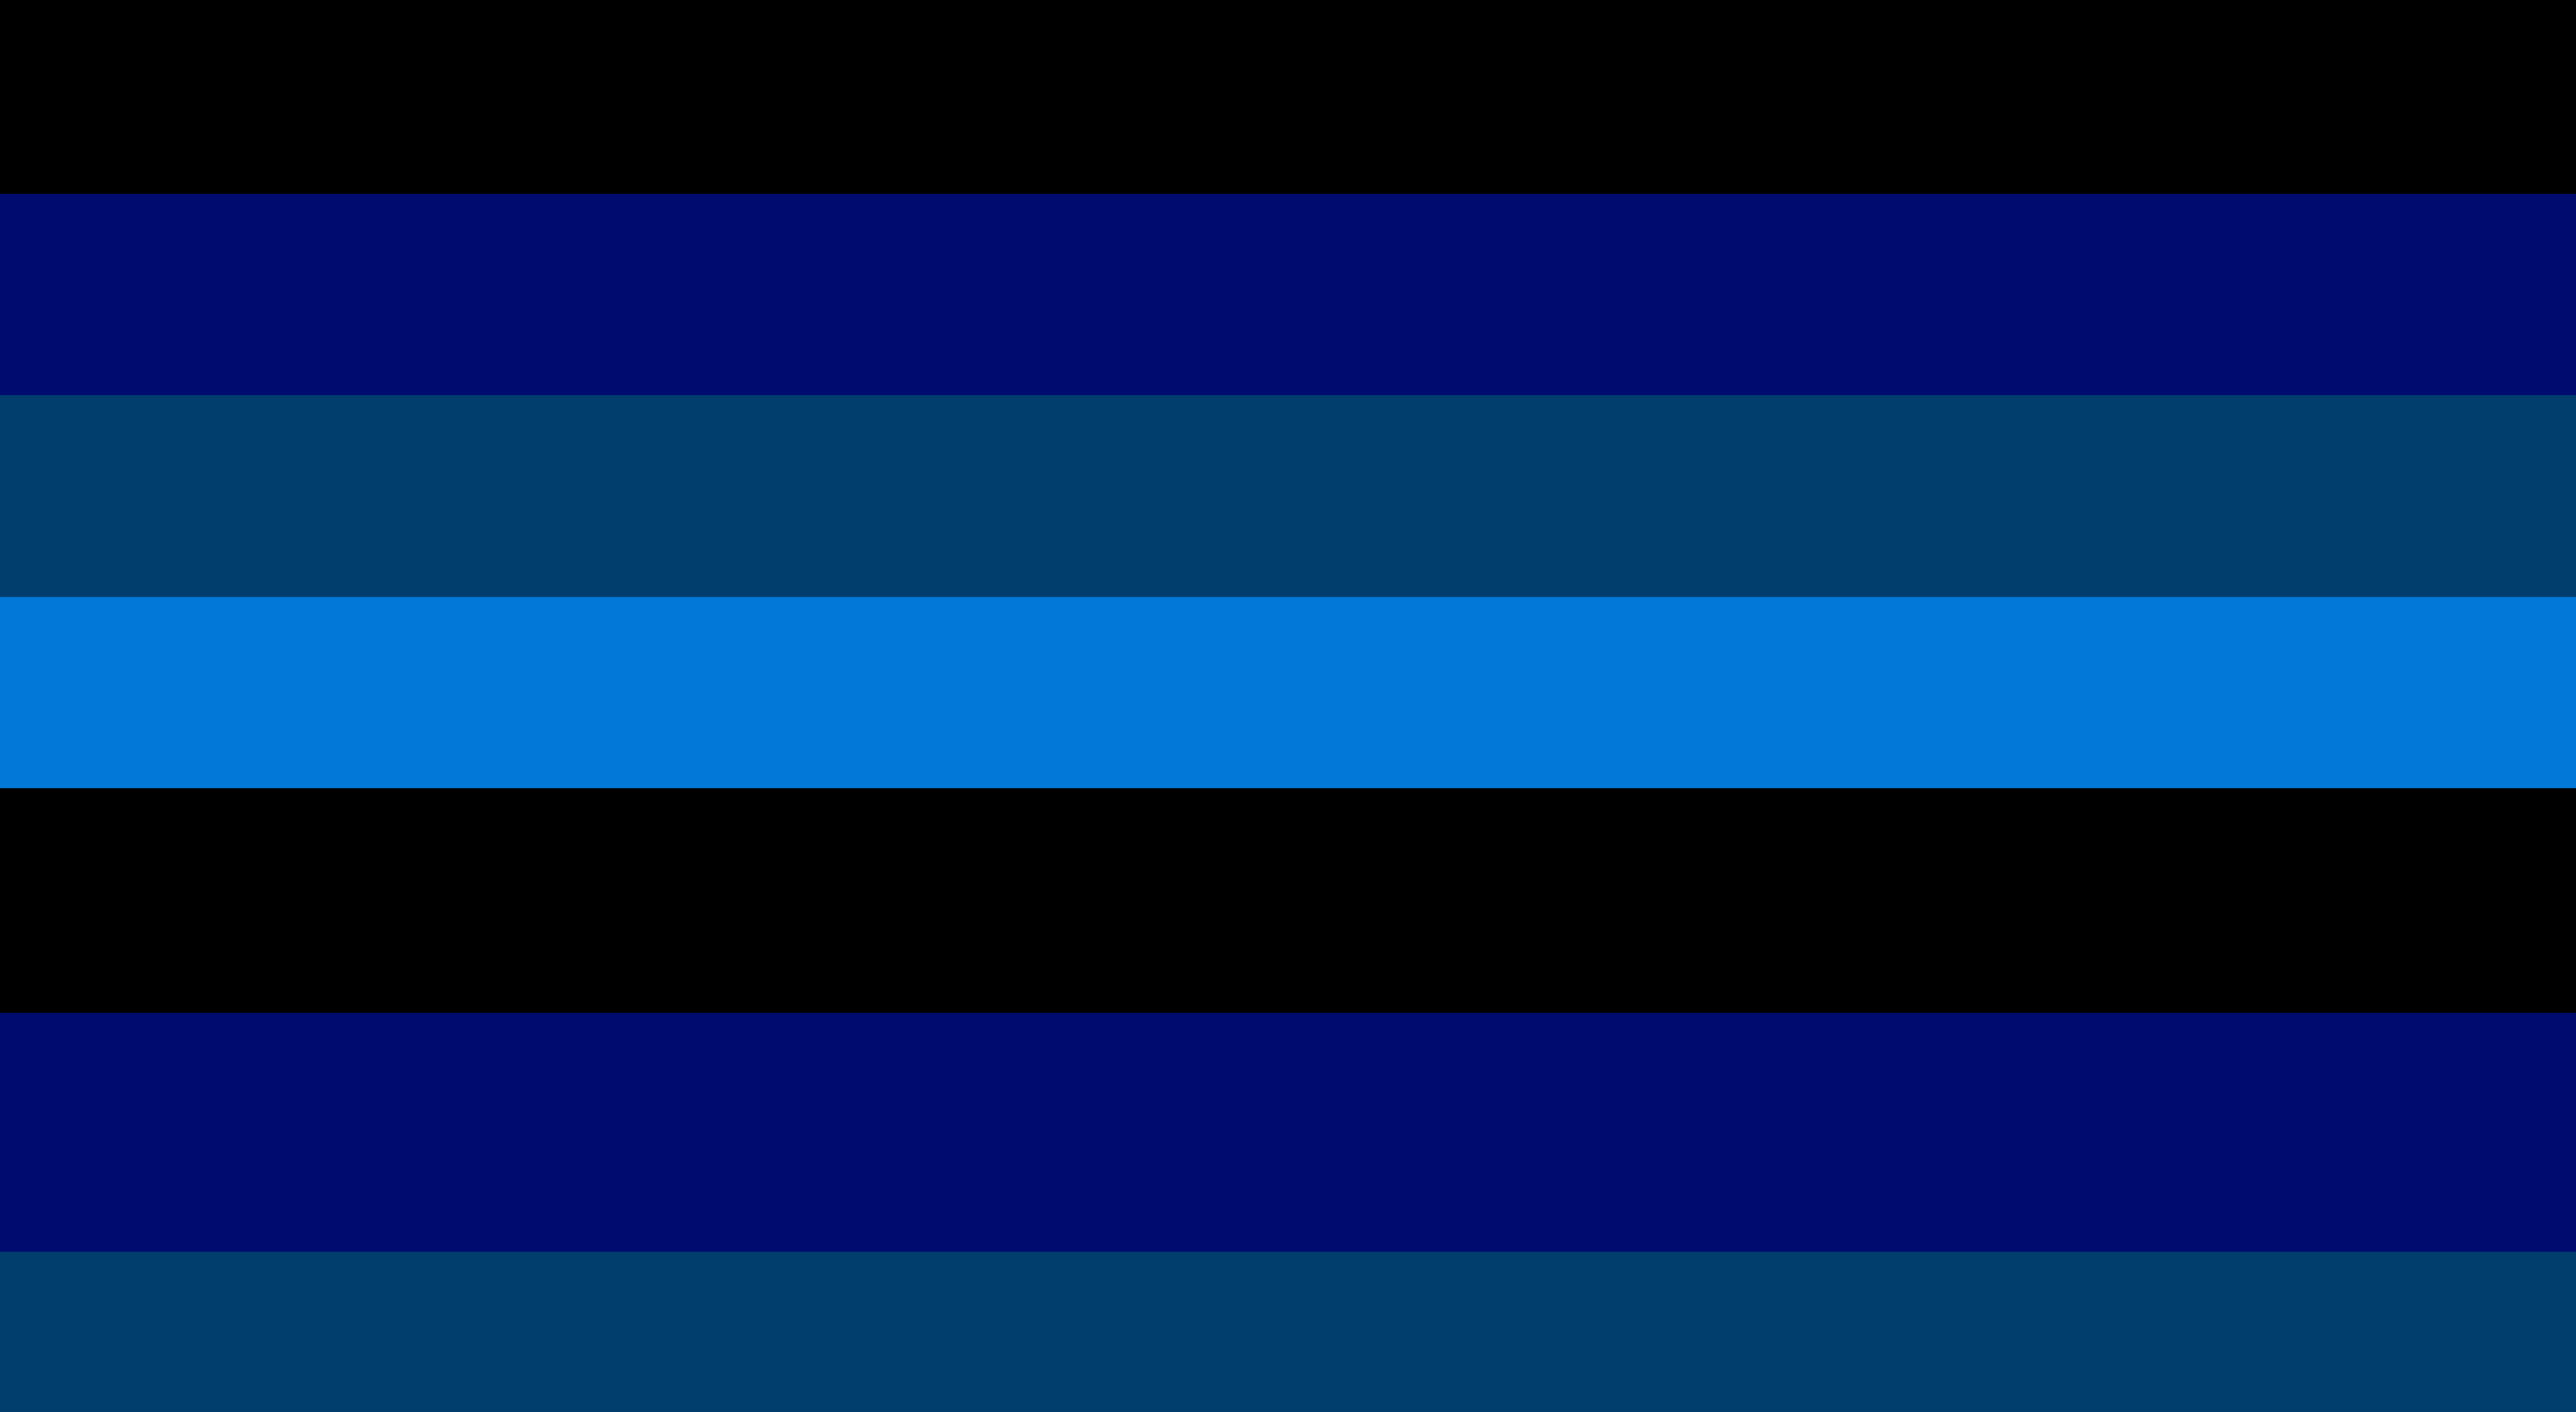
\includegraphics[width=0.3\textwidth]{C7H16.png}}  
  \caption{Droplets colored by mass fractions}
  \label{Droplets colored by mass fractions}
\end{figure}
\section{Your own evaporation model}
To copy and create your own evaporation model follow these step-by-step instructions.

\subsection{Copy the dieselFoam solver}
Copy the dieselFoam solver to your working directory.
\begin{verbatim}
mkdir -p $WM_PROJECT_USER_DIR/applications/solvers/combustion
cp -r $FOAM_SOLVERS/combustion/dieselFoam $WM_PROJECT_USER_DIR\
/applications/solvers/combustion/mydieselFoam     	
\end{verbatim}
\noindent
Rename solver to mydieselFoam.
\begin{verbatim}
cd $WM_PROJECT_USER_DIR/applications/solvers/combustion/mydieselFoam/Make
\end{verbatim}
\noindent
Change in the \verb+/Make/files+ so it reads.
\begin{verbatim}
dieselFoam.C

EXE = $(FOAM_USER_APPBIN)/mydieselFoam
\end{verbatim}
\noindent
Change in the \verb+/Make/options+ so the second line reads.
\begin{verbatim}
-I$(LIB_SRC)/../applications/solvers/combustion/dieselEngineFoam \
\end{verbatim}


\subsection{Copy the dieselSpray library}
Copy the \verb+src/lagrangian/dieselSpray+ dictionary to your user dictionary and rename it to
\newline \noindent
\verb+mydieselSpray+. 

\begin{verbatim}
cd $WM_PROJECT_DIR
cp -riuv --parents --backup src/lagrangian/dieselSpray \
$WM_PROJECT_USER_DIR
cd $WM_PROJECT_USER_DIR/src/lagrangian
mv dieselSpray mydieselSpray
\end{verbatim} 
\noindent
Copy the \verb+standardEvaporationModel+ dictionary to \verb+my_standardEvaporationModel+.

\begin{verbatim}
cd $WM_PROJECT_USER_DIR/src/lagrangian/mydieselSpray/spraySubModels/evaporationModel 
cp -r standardEvaporationModel my_standardEvaporationModel 
\end{verbatim} 
\noindent
Change \verb+standardEvaporationModel+ to \verb+my_standardEvaporationModel+ in the \verb+.C+ and \verb+.H+ file using \verb+sed+ and rename the files to \verb+my_standardEvaporationModel+. 

\begin{verbatim}
cd $WM_PROJECT_USER_DIR/src/lagrangian/mydieselSpray/spraySubModels/evaporationModel
cd  my_standardEvaporationModel
sed s/standardEvaporationModel/my_standardEvaporationModel/g \
standardEvaporationModel.C >my_standardEvaporationModel.C
sed s/standardEvaporationModel/my_standardEvaporationModel/g \
standardEvaporationModel.H >my_standardEvaporationModel.H
rm standardEvaporationModel.C standardEvaporationModel.H
\end{verbatim}
\noindent
Add \verb+my_standardEvaporationModel.C+ to the list of evaporation models in \newline \noindent
\verb+/mydieselSpray/Make/files+ line 59.
\begin{verbatim}
.
.
$(evaporationModels)/saturateEvaporationModel/saturateEvaporationModel.C
$(evaporationModels)/my_standardEvaporationModel/my_standardEvaporationModel.C
\end{verbatim}
\noindent
Also, change the name of the library at the bottom of the \verb+/mydieselSpray/Make/files+ file to
\begin{verbatim}
LIB = $(FOAM_USER_LIBBIN)/libmydieselSpray
\end{verbatim}

\subsection{Adding mydieselSpray library to mydieselFoam solver}
Go to your \verb+mydieselFoam+ directory 
\begin{verbatim}
cd $WM_PROJECT_USER_DIR/applications/solvers/combustion/mydieselFoam/Make
\end{verbatim}
Open the \verb+options+ file and change line 6 from 
\begin{verbatim}
-I$(LIB_SRC)/lagrangian/dieselSpray/lnInclude \
\end{verbatim}
to:
\begin{verbatim}
-I$(WM_PROJECT_USER_DIR)/src/lagrangian/mydieselSpray/lnInclude \
\end{verbatim}
At the end of the \verb+options+ file change so it reads:
\begin{verbatim}
-lpdf \
-L$(WM_PROJECT_USER_DIR)/lib/$(WM_OPTIONS) \
-lmydieselSpray
\end{verbatim}
\subsection{Update case files}
Update the \verb+sprayProperties+ so it includes the coefficients for\newline \noindent your evaporation model in \verb+aachenBomb/constant/sprayProperties+. 
\begin{verbatim}
cd $FOAM_RUN/aachenBomb/constant
\end{verbatim}
Edit \verb+sprayProperties+ so the evaporation model is set to:
\begin{verbatim}
evaporationModel my_standardEvaporationModel;
\end{verbatim}
Also, add model coefficients for your evaporation model in then \verb+sprayProperties+ file  

\begin{verbatim}
my_standardEvaporationModelCoeffs
{ 
    evaporationScheme explicit; 
    preReScFactor   0.6; 
    ReExponent      0.5; 
    ScExponent      0.333333; 
}
\end{verbatim}
\subsection{Customizing the evaporation model}
Go back to the \verb+my_standardEvaporationModel+ directory.
\begin{verbatim}
cd $WM_PROJECT_USER_DIR/src/lagrangian/mydieselSpray/spraySubModels/\
evaporationModel/my_standardEvaporationModel
\end{verbatim} 
Take a closer look in \verb+my_standardEvaporationModel.C+. On line 98 to 104 it reads,
\begin{verbatim}
scalar my_standardEvaporationModel::Sh
(
    const scalar ReynoldsNumber,
    const scalar SchmidtNumber
) const
{
    return 2.0 + preReScFactor_*pow(ReynoldsNumber,ReExponent_)\ 
    *pow(SchmidtNumber,ScExponent_);
}
\end{verbatim} 
That is, the Sherwood number is calculated according to the \textit{Ranz-Marshall} correlation \footnote{Multiphase flows with droplets and particles, Crowe et al. (1998) CRC Press LLC}, see equation \ref{Sh}, observe that the \verb+my_standardEvaporationModelCoeffs+ are used here.
\begin{equation}
\label{Sh}
	Sh=2+0.6Re_{r}^{0.5}Sc^{0.33333}
\end{equation}
Where $Sh$ is the Sherwood number, $Re_{r}$ relative Reynold number and $Sc$ Schmidt number.
\newline
\noindent
In this tutorial we will make changes to the evaporation time, located in \newline\noindent
\verb+my_standardEvaporationModel.C+, on line 142 to 163. 
\begin{verbatim}
scalar Xratio = (Xs - Xf)/max(SMALL, 1.0 - Xs);

if (Xratio > 0.0)
{
    lgExpr = log(1.0 + Xratio);
}

scalar denominator =
6.0 * massDiffusionCoefficient
* Sh(ReynoldsNumber, SchmidtNumber)
* rhoFuelVapor * lgExpr;

if (denominator > SMALL)
{
time = max(VSMALL, liquidDensity * pow(diameter, 2.0)/denominator);
}

return time;
\end{verbatim}
We want the evaporation time $\tau_{m}$ to be calculated by a $D^2$-law showed in equations \ref{lambda} and \ref{taum}
\begin{equation}
\label{lambda}
	\lambda =\frac{4Sh \rho_{c} D_v}{\rho_{d}} \left( \omega_{A,s}-\omega_{A,\infty} \right)
\end{equation}
Where $\lambda$ is the evaporation constant, $\rho_{c}$ film density, $\rho_{d}$ droplet density, $D$ diameter, $D_v$ diffusion coefficient for species $A$, $\omega_{A,s}$ mass fraction of species $A$ at the droplet surface and $\omega_{A,\infty}$ for the free stream.  
\begin{equation}
\label{taum}
	\tau_{m}=\frac{D^{2}}{\lambda}
\end{equation}
Make changes in the \verb+my_standardEvaporationModel.C+ file, according to the equations showed. Start by removing \verb+scalar lgExpr = 0.0;+ on line 123.
\newline \noindent
Edit the \verb+my_standardEvaporationModel.C+ file and change \verb+scalar Xratio+ and \verb+scalar denominator+. 
\newline
\noindent
Remove the \verb+if (Xratio > 0.0)+ statement completely.
\begin{verbatim}
scalar Xratio = (Xs - Xf);

scalar denominator =
4.0 * massDiffusionCoefficient
* Sh(ReynoldsNumber, SchmidtNumber)
* rhoFuelVapor*Xratio;

if (denominator > SMALL)
{
   time = max(VSMALL, liquidDensity * pow(diameter, 2.0)/denominator);
}

return time;
\end{verbatim}
\subsection{Compile library and solver}
Compile the \verb+mydieselSpray+ library and your solver. 
\begin{verbatim}
cd $WM_PROJECT_USER_DIR/src/lagrangian/mydieselSpray
wclean
rm -r lnInclude
rm -r Make/linux*
wmake libso
 
cd $WM_PROJECT_USER_DIR/applications/solvers/combustion/mydieselFoam
wclean
rm -r Make/linux*
wmake
\end{verbatim}
\subsection{Running the case}
Start the solver with \verb+mydieselFoam+ and post in ParaView as described in section \ref{Post-processing in ParaView}.
When the solver starts check that your evaporation model is being used.
\begin{verbatim} 
cd $FOAM_RUN/aachenBomb
blockMesh
mydieselFoam  
\end{verbatim}

\chapter*{Study questions}
\begin{enumerate}
\item How do you ...
\item What is the purpose of...
\item ...
\end{enumerate}

\end{document}
